\documentclass[../main.tex]{subfiles}
\graphicspath{{\subfix{../figures/}}}
\begin{document}
The system which was studied in this thesis is essentially given by \cref{fig:model}, with a few assumptions and modifications. To reduce the dimension of the parameter space, a fixed tunneling rate $\Gamma$ and a variable tunneling detuning $\delta\Gamma$ are introduced. The four tunneling rates in terms of $\Gamma$ and $\delta\Gamma$ are assumed to be symmetrically given by \cref{fig:model}. It is also assumed that each dot is restricted to be either empty or contain one (spinless) electron in the ground state of the dot. The energy of the ground state is given by a fixed gate voltage $V_\text{G}=0$ and a variable energy detuning $\delta\epsilon$: $\epsilon_{1/2} = -V_\text{G} \pm \delta\epsilon$. Furthermore, the temperatures of the leads $T_\text{L}=T_\text{R}=10\Gamma$, the chemical potentials $\mu_\text{L/R} = \pm V_\text{SD}/2$, the bias voltage $V_\text{SD} = 300\Gamma$, and the charging energy $U = 250\Gamma$, are all treated as constants. The charging energy being the extra energy needed to enter a quantum dot if the other dot is already occupied due to Coulomb interaction. This leaves the two tuning parameters, $\delta\Gamma$ and $\delta\epsilon$, as the only parameters of the system, resulting in a two dimensional parameter space. 

\begin{figure}[H]
    \centering
    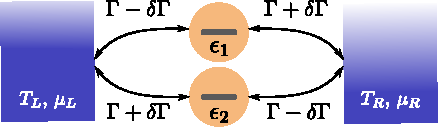
\includegraphics[width=0.8\linewidth]{figures/model.pdf}
    \caption{hej}
    \label{fig:model}
\end{figure}

The full Hamiltonian of the system is given by $\hat H = \hat H_\text{QD} + \hat H_\text{leads} + \hat H_\text{tunneling}$ where the three terms correspond to the quantum dot, lead, and tunneling Hamiltonians. By considering all the tunneling processes, these terms can be modeled by
\begin{equation}
    \begin{aligned}
        \hat H_\text{QD} &= (\epsilon - \delta\epsilon) \hat d_1^\dag \hat d_1  +  (\epsilon + \delta\epsilon)\hat d_2^\dag \hat d_2 + U\hat d_1^\dag \hat d_1 \hat d_2^\dag \hat d_2, \\
        \hat H_\text{leads} &= \sum_{k} (E_{L,k} \hat c_{L,k}^\dag \hat c_{L,k}  + E_{R,k} \hat c_{R,k}^\dag \hat c_{R,k}), \\
        \hat H_\text{coup} &= \sum_k (t_{L,1} \hat d_1^\dag \hat c_{L,k} + t_{L,2} \hat d_2^\dag \hat c_{L,k} + t_{R,1} \hat d_1^\dag \hat c_{R,k} + t_{R,2} \hat d_2^\dag \hat c_{R,k}) + \text{H.c},
    \end{aligned}
\end{equation}
where $\hat d_{1/2}^\dag$ creates an electron in dot 1 or 2, and $\hat c_{L/R,k}^\dag$ creates an electron in the left or right lead with quantum number $k$ and energy $E_{L/R,k}$. The tunneling amplitudes $t_{L/R,1/2}$ are directly related to the corresponding tunneling rates $\Gamma_{L/R,1/2}$. 

To be able to simulate the dynamics of the system, a couple more approximations have to be made regarding the coupling between the dots and the leads. (reasonable assumptions?) The first is to assume that the strength of the coupling between the system and the environment is weak. It is therefore possible to treat the interaction perturbatively in terms of the tunneling rate $\Gamma$. The second main approximation is to assume that the interaction between the system and the environment is Markovian. A Markovian process is one in which the next time step only depends on the current state of the system. In a quantum dot system, this can be interpreted to mean that the leads "forget" that they have lost or gained an electron, right after the tunneling process has happened. Since the number of electrons in the leads typically is large, this can be a reasonable approximation for such systems.

These last two assumptions are made to motivate the use of a common tool used to simulate open quantum systems, the Lindblad master equation. The next two sections will introduce the theory necessary to understand its uses and origin.

\end{document}
